\documentclass[dcc]{fcfmcourse}
\usepackage{teoria}
\usepackage[utf8x]{inputenc}
\usepackage[nocenter]{qtree}
\usepackage{hyperref}

\renewcommand{\figurename}{Figura.}

\title{Tarea 3: Pila de Arena Optimizada}
\course[CC3001]{Algoritmos y Estructuras de Datos}
\professor{Nelson Baloian}
\professor{Patricio Poblete}
\assistant{Gabriel Azócar}
\assistant{Manuel Cáceres}
\assistant{Michel Llorens}
\assistant{Sergio Peñafiel}
% Si pasas el comando usedate a la clase, la fecha aparecerá bajo la lista de auxiliares.
% Puedes usar el formato de fecha por defecto de latex (y traducirla usando babel)
% o puedes escribir lo que quieras con el comando \date.
% \date{1 de Septiembre, 2015}


\begin{document}
\maketitle
\vspace{-2ex}
\begin{center}
Fecha de Entrega: 8 de Mayo  23:59hrs \\
\end{center}


\section{Introducción}

En el problema resuelto en la Tarea 1: ``Pilas de Arena'' fuimos capaces de generar el proceso de estabilización de la matriz, recorriéndola tantas veces como sea necesario hasta que ya no se encontraran casilleros de \textit{desborde}. Recordemos que un casillero de \textit{desborde} es aquel en el cual se encuentran apilados 4 o más granos de arena.

\begin{figure}[!ht]
    \centering
    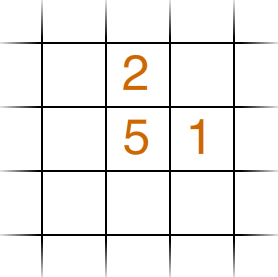
\includegraphics[scale=0.45]{imagenes/gridex1.png}
\end{figure}

Estos casilleros deben \textit{desbordar} dejando un grano en cada una de las celdas vecinas (arriba, abajo, derecha e izquierda).

\begin{figure}[!ht]
    \centering
    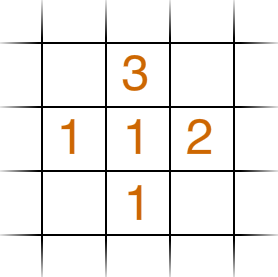
\includegraphics[scale=0.45]{imagenes/gridex2.png}
\end{figure}

El problema de revisar la matriz en busca de casilleros de \textit{desborde} es que muchas de las casillas de la matriz no necesitan ser \textit{desbordados} por lo que se gasta innecesariamente tiempo de computo.\\

\begin{figure}[!ht]
    \centering
    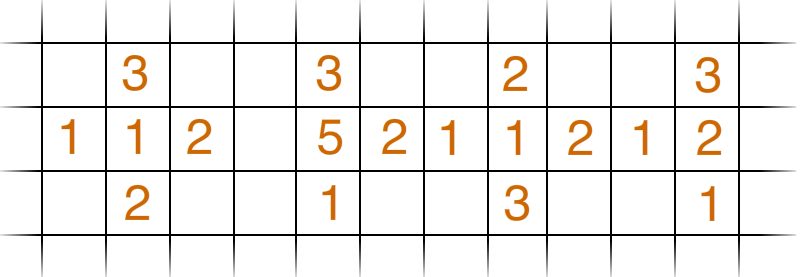
\includegraphics[scale=0.4]{imagenes/sandpilelarge.png}
    \caption{Si el algoritmo revisa todas las casillas de la matriz al revisar la fila de al medio solo \textit{desbordará} la que tiene un 5 y las demás serán revisadas innecesariamente.}
\end{figure}

En esta tarea se estudiará e implementará un tipo de dato abstracto (TDA) adicional a la matriz, que permita insertar y eliminar casillas en tiempo constante, identificando las casillas de \textit{desborde} sin tener que procesar las que no lo son.\\ 

El TDA que pedimos implementar es la \textbf{Pila}, que se rige según el principio ``LIFO'', es decir, el último elemento insertado es el primero extraído. Como fue visto en cátedras este TDA puede ser implementado usando un arreglo redimensionable o con una lista enlazada, usted puede escoger cualquiera de ellas para su implementación.\footnote{Más detalle del funcionamiento de la \textbf{Pila} en los apuntes : \\ \href{https://users.dcc.uchile.cl/~bebustos/apuntes/cc3001/TDA/\#2}{https://users.dcc.uchile.cl/$\sim$bebustos/apuntes/cc3001/TDA/\#2}.}
\begin{figure}[!ht]
    \centering
    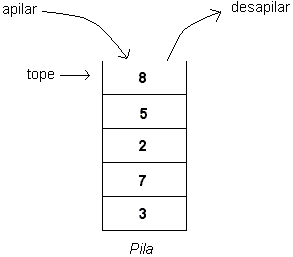
\includegraphics[scale=0.5]{imagenes/pila.png}
    \caption{Imagen ilustrativa del funcionamiento y operaciones de una \textbf{Pila}}
\end{figure}
\section{Implementación}
\subsection{El TDA Pila}
Debe implementar un TDA \texttt{Pila} en el archivo \textbf{Pila.java} con las siguientes operaciones:

\begin{itemize}

\item Un constructor, \texttt{Pila()}:

Construye una representación para el TDA inicialmente sin elementos, debe inicializar todo lo necesario para que el resto de las operaciones funcionen correctamente.

\item \texttt{bolean estaVacia()}:

Retorna \texttt{true} si la \texttt{Pila} no tiene elementos y \texttt{false} en caso contrario.

\item \texttt{void apilar(int i, int j)}:

Debe poner en la \texttt{Pila} los índices de casilla $(i,j)$.

\item \texttt{int[] desapilar()}:

Debe extraer los índices de casilla de la \texttt{Pila}, estos índices deben ser retornados en un arreglo de 2 elementos.

\end{itemize}


\subsection{Uso del TDA, Pila de Arena Optimizada}
En el archivo \textbf{PilaArenaOptimizada.java} debe realizar el mismo procedimiento que realizó en su Tarea 1 en el archivo \textbf{PilaArena.java} (misma forma de recibir input, de nuevo posee la clase \textbf{Ventana} para visualizar sus resultados). También mantenga la matriz de las casillas, pero esta vez para identificar los casilleros de \textit{desborde} utilice la \textbf{Pila} antes explicada. Comience insertando los índices de la casilla del centro, luego mientras hayan elementos en la \textbf{Pila}, \textit{desbórdelos} e inserte las casillas \textit{desborde} que se creen después de este proceso. De este modo, si por ejemplo estoy procesando el 5 central en
\begin{figure}[!ht]
    \centering
    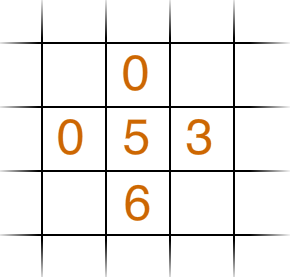
\includegraphics[scale=0.45]{imagenes/gridex3.png}
\end{figure}
%   | 0 |
% 0 | 5 | 3
%   | 6 |
\\y aplico el \textit{desborde} obtengo
\begin{figure}[!ht]
    \centering
    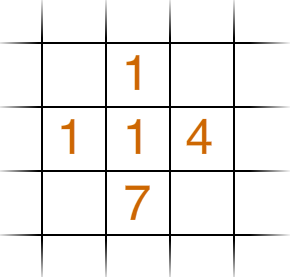
\includegraphics[scale=0.45]{imagenes/gridex4.png}
\end{figure}
%   | 1 |
% 1 | 1 | 4
%   | 7 |
\newpage
, por lo que:
\begin{itemize}
    \item No vuelvo a insertar la casilla central al TDA, pues ya no es una casilla de \textit{desborde}.
    \item Inserto la casilla de la derecha al TDA, pues pasa a ser casilla de \textit{desborde}.
    \item La casilla de abajo no debo insertarla al TDA, pues antes de \textit{desbordar} la central esta ya era una casilla de \textit{desborde} encontrándose en el TDA.
\end{itemize}

\subsection{Tratamiento del caso borde}
Se solicita que el tratamiento del caso borde se realice utilizando matrices de tamaño suficientemente grande. Si el input es de tamaño $N$ utilice matrices de tamaño $\sqrt{N}\times\sqrt{N}$.
\section{Experimentación}

Compare los tiempos de esta implementación con la realizada en la Tarea 1 para diferentes tamaños de inputs, tome 10 valores de $N$ equiespaceados  $\in [10^3, 10^5]$, investigue si realmente esta nueva implementación es más rápida, grafique ambas funciones y compare.
\section{Condiciones de Entrega}

\begin{itemize}
    \item Esta tarea debe ser resuelta en Java.
    \item Es obligatoria la entrega de un informe en formato pdf junto con su tarea (Ver siguiente sección).
    \item Esta tarea es de carácter individual, cualquier caso de copia se evaluará con la nota mínima.
    \item No olvide subir a U-cursos todos los archivos necesarios para que su tarea funcione correctamente.
    \item Debe subir los archivos de código fuente (*.java). Los archivos compilados (*.class) no serán evaluados.
    \item Cualquier duda respecto a la tarea puede ser consultada usando el foro del curso.
    \item \textbf{NO} se aceptarán atrasos.
\end{itemize}


\section{Informe}

El informe debe describir el trabajo realizado, la solución implementada, los resultados obtenidos
y las conclusiones o interpretaciones de estos. Principalmente debe ser breve, describiendo cada uno
de los puntos que a continuación se indican:

\begin{itemize}
    \item \textbf{Portada:} Indicando número de la tarea, fecha, autor, email, código del curso, etc.
    \item \textbf{Introducción:} Descripción breve del problema y su solución.
    \item \textbf{Análisis del problema:} Exponga en detalle el problema, los supuestos que pretende ocupar, casos de borde y brevemente la metodología usada para resolverlo.
    \item \textbf{Solución del problema:} Indique claramente los pasos que siguió para llegar a la solución
del problema. Muestre mediante figuras y ejemplos qué es lo que realiza su código. Evite
copiar todo el código fuente en el informe, sin embargo, puede mostrar las partes relevantes
de éste.
\item \textbf{Modo de uso:} Explicando brevemente cualquier dato necesario para la compilación y
ejecución de su programa.
\item \textbf{Resultados:} Muestre ejemplos de entradas y salidas de su programa. Además muestre el resultado de los experimentos, las distintas figuras y gráficos obtenidos.
\item \textbf{Discusión:} 
\begin{itemize}
    \item Discuta sobre la complejidad de los métodos del TDA, en especial argumente porque sus implementaciones cumplen con las restricciones de tiempo. 
    \item Discuta si esta solución es más rápida que la obtenida en la Tarea 1, si es así diga si esta es significativa, si no lo fue de argumentos del por qué de esta situación. Justifique además los gráficos obtenidos en la sección de resultados.
\end{itemize}



\end{itemize}

\end{document}